\section{An Algorithm for Finding Bugs}
In order to detect resource manipulation bugs, I will present an algorithm for detecting these bugs utilizing the definitions presented by Abal et. al \cite{EffectiveBugFinding}. This section will present my definitions of \textit{monitor templates} as finite state machines operating on \textit{effects} on \textit{regions}, allowing the definition of bug behaviour and the detection of such behaviour. 

\newpar A finite state machine is a tuple $(\sum, S, s_0, \delta, F)$, where $\sum$ is an alphabet, $S$ is a finite non-empty set of states, $s_0$ is an element of $S$ and initial state, $\delta$ is the state-transition function $\delta: S \times \sum \rightarrow S$ and $F$ is the possibly empty set of final states and a subset of $S$. I will use such state machines to represent the code under analysis and the properties I wish to detect in input source files. 

\subsection{Monitor Templates}
\label{monitor-template-section}
\noindent I use monitor automata to analyze the control flow of a given input source file and detect whether possible bug are present in. A monitor automaton changes state based on what is happening in the control flow of the program. When the automaton reaches an error state, then a possible bug has been discovered. The effect analysis provided by EBA allows monitoring which effects program points have, and monitor automata can then monitor these effects in order to determine whether possible bugs are present. 

\newpar EBA infers what effects happen on a memory region, which is an abstract variable or value in the heap. Monitor automata track effects happening on a given region in order to determine whether they could be manifesting buggy behaviour. Both effects and regions must be tracked. For example, it is common to have multiple locks on different regions within programs, but a lock on one region followed by a lock on a different region does not neccesarily mean that a locking bug is present unless these locks happen consequently on the same region. Monitor templates are defined formally as follows. 

\newpar Given a region variable $\rho$, a monitor template is defined as the tuple $X_\rho (\sum, S, s_0, \delta, F, E)$ where $\sum$ is the alphabet of effects registered on memory objects represented by a region $\rho$, $S$ is a finite non-empty set of states, $s_0$ an initial state and an element of $S$, $\delta$ is the state-transition function $\delta: S \times \sum \rightarrow S$, $F$ is the non-empty set of final states and a subset of $S$, $E$ is the non-empty set of error states, and a subset of $F$. In other words, $X_\rho (\sum, S, s_0, \delta, F)$ is a finite state machine over regions and effects, augmented with the set of error states $E$. An illustration of such a monitor template can be seen in Figure \ref{double-unlock-automata-intro}.

\newpar From this definition, I distinguish two kinds of monitor templates: \textit{long-term} and \textit{short-term}. \textit{Short-term} templates will monitor effects happening on a region only until a final state or error state is reached. \textit{Long-term} templates operate as \textit{short-term} templates, though they only include a single final state, which is the error state. They will therefore monitor indefinititely until only an error-state is found; no early temrination is possible. This distinction is made since early termination of monitors might result in performance improvements in the implementation of these monitors, since it may especiaally reduce the number of monitors active in the analyzers' memory. 

\begin{figure}[H]
    \centering
    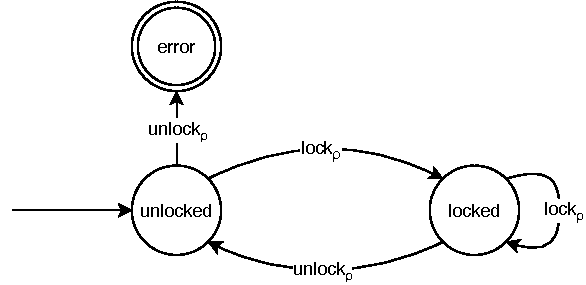
\includegraphics[width=0.5\textwidth]{algorithm/figures/double-unlock}
    \caption{An illustration of a monitor template.}
    \label{double-unlock-automata-intro}
\end{figure}

\newpar I will present several examples of these monitors in the following sections. Though these are examples, they are important since the implementation of the monitors follows these examples. 

\newpar Our monitors operate on the set of possible effects of a statement in the Control-flow Graph. EBA allows defining new effects tracking a host of different operation. In this thesis I will only be using the following effects, defined as $E = \{$\texttt{alloc}, \texttt{free}, \texttt{read}, \texttt{write}, \texttt{uninit}, \texttt{call}, \texttt{lock}, \texttt{unlock}$\}$ by Abal \cite{EffectiveBugFinding}. The effects and what they represent can be seen in Table \ref{effect-table}.

\begin{table}[H]
    \centering
    \begin{tabular}{ll}
        \texttt{alloc}  & The allocation of a memory location                   \\
        \texttt{free}   & The freeing of a memory location                      \\
        \texttt{read}   & The reading of a memory location                      \\
        \texttt{write}  & The writing to a memory location                      \\
        \texttt{uninit} & Indicating that a memory location is uninitialized    \\
        \texttt{call}   & The call of a function                                \\
        \texttt{lock}   & The locking of a memory location                      \\
        \texttt{unlock} & The unlocking of a memory location    
    \end{tabular}
    \caption{Effects and what they represent.}
    \label{effect-table}
\end{table}

\subsubsection*{Short-term Double-lock Monitor Template}

\begin{figure}[H]
    \centering
    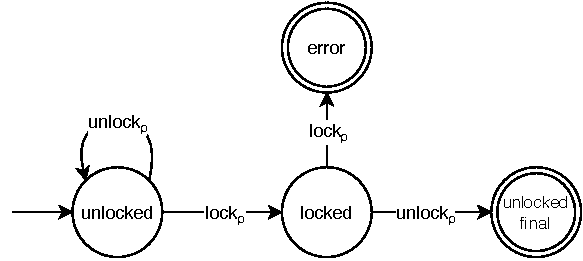
\includegraphics[width=0.5\textwidth]{algorithm/figures/double-lock-short-term}
    \caption{An illustration of a short-term double-lock monitor template.}
    \label{double-lock-automata-short-term}
\end{figure}

A double-lock monitor detects two consecutive locks on a memory location with no unlock in between them leading to an infinite spinlock. Given a region $\rho$, a double-lock monitor template is defined as the tuple $(\sum, S, s_0, \delta, E, F)$ where: 

\begin{itemize}
    \item $\sum = \{lock_\rho, unlock_\rho\}$, a subset of $E$
    \item $S = \{ locked_\rho, unlocked_\rho, error_\rho \}$
    \item $s_0 = unlocked_\rho$ 
    \item $\delta =$ the relation $\{(unlocked_\rho, lock_\rho, locked_\rho), (locked_\rho, unlock_\rho, unlocked_\rho), \\
    (locked_\rho, lock_\rho, error_\rho), (unlocked_\rho, unlock_\rho, unlocked_\rho)\}$ 
    \item $E = \{ error_\rho \}$  
    \item $F = \{ unlocked_\rho, error_\rho \}$
\end{itemize}

\noindent It is worth noting that this is a \textit{short-term} monitor, as $F \neq E$. This monitor will therefore terminate when encountering a legal use of locks followed by an unlock. An illustration of this monitor template can be seen in Figure \ref{double-lock-automata-short-term}. 

\subsubsection*{Long-term Double-unlock Monitor Template}

\begin{figure}[H]
    \centering
    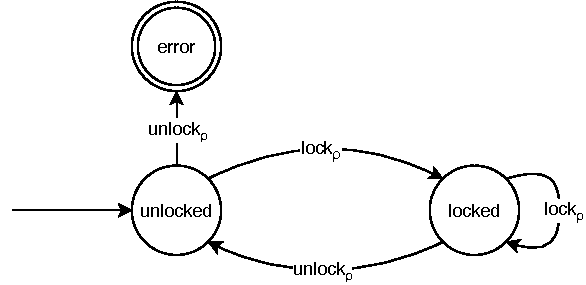
\includegraphics[width=0.5\textwidth]{algorithm/figures/double-unlock}
    \caption{An illustration of a long-term double-unlock monitor template.}
    \label{double-unlock-automata}
\end{figure}

A double-unlock monitor detects two consecutive unlocks on a memory location with no lock in between them, leading to undefined behaviour. Given a region $\rho$, a double-unlock monitor template is defined as the tuple $(\sum, S, s_0, \delta, E, F)$ where: 

\begin{itemize}
    \item $\sum = \{unlock_\rho, lock_\rho\}$, a subset of $E$
    \item $S = \{ locked_\rho, unlocked_\rho, error_\rho \}$
    \item $s_0 = unlocked_\rho$ 
    \item $\delta =$ the relation $\{(locked_\rho, unlock_\rho, unlocked_\rho), (locked_\rho, lock_\rho, locked_\rho), \\
        (unlocked_\rho, lock_\rho, locked_\rho), (unlocked_\rho, unlock_\rho, error_\rho)\}$ 
    \item $E = \{ error_\rho \}$
    \item $F = E$
\end{itemize}

\noindent It is worth noting that this is a \textit{long-term} monitor, as $F = E$. An illustration of this monitor template can be seen in Figure \ref{double-unlock-automata}. 

\subsubsection*{Long-term Double-free Monitor Template}

\begin{figure}[H]
    \centering
    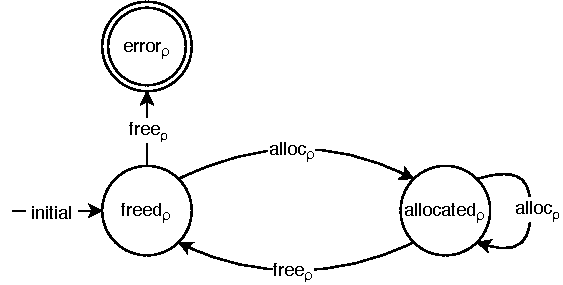
\includegraphics[width=0.5\textwidth]{algorithm/figures/double-free}
    \caption{An illustration of a long-term double-free monitor template.}
    \label{double-free-automata}
\end{figure}

A double-free monitor detects two consecutive frees on a memory location with no allocation in between them, potentially leading to modification of unexpected memory locations. Given a region $\rho$, a double-free monitor template is defined as the tuple $(\sum, S, s_0, \delta, E, \\F)$ where: 

\begin{itemize}
    \item $\sum = \{free_\rho, alloc_\rho\}$, a subset of $E$
    \item $S = \{ allocated_\rho, freed_\rho, error_\rho \}$
    \item $s_0 = freed_\rho$ 
    \item $\delta =$ the relation $\{(freed_\rho, alloc_\rho, allocated_\rho), (allocated_\rho, free_\rho, freed_\rho), \\
    (freed_\rho, free_\rho, error_\rho), (allocated_\rho, alloc_\rho, allocated_\rho)\}$ 
    \item $E = \{ error_\rho \}$  
    \item $F = E$
\end{itemize}

An illustration of this monitor template can be seen in Figure \ref{double-free-automata}. 

\subsubsection*{Short-term Use-before-init Monitor Template}

\begin{figure}[H]
    \centering
    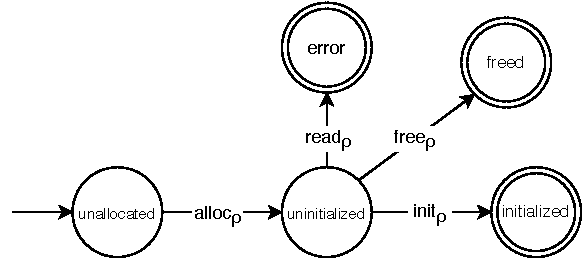
\includegraphics[width=0.4\textwidth]{algorithm/figures/use-before}
    \caption{An illustration of a short-term use-before-init monitor template.}
    \label{use-before-automata}
\end{figure}

A use-before init monitor detects usage of a memory location before the location has been initialized, possibly leaving the resource in an unexpected state when it is accessed or used. Given a region $\rho$, a use-before-init monitor template is defined as the tuple $(\sum, S, s_0, \delta, E, \\F)$ where: 

\begin{itemize}
    \item $\sum = \{read_\rho, init_\rho\}$, a subset of $E$
    \item $S = \{ uninitialized_\rho, initialized_\rho, error_\rho \}$
    \item $s_0 = uninitialized_\rho$ 
    \item $\delta =$ the relation $\{(uninitialized_\rho, init_\rho, initialized_\rho), (uninitialized_\rho, read_\rho, error_\rho)\}$ 
    \item $E = \{ error_\rho \}$  
    \item $F = \{ error_\rho, initialized_\rho \}$
\end{itemize}

An illustration of this monitor template can be seen in Figure \ref{use-before-automata}. 

\subsection{Control Flow}

EBA provides a representation of the control flow of the input source files which is utilized in order to detect bugs. EBA generates a tree structure of the input with path in this tree structure modeling a possible execution path containing information about the modelled statements. 

\newpar The control flow graph of a program can be seen as a finite state machine $(\sum, S, s_0, \delta, F)$, where $\sum$ is the alphabet, $S$ is a finite non-empty set of states, $s_0$ is an element of $S$ and initial state, $\delta$ is the state-transition function $\delta: S \times \sum \rightarrow S$ and $F$ is the possibly empty set of final states and a subset of $S$. 

\newpar The control flow generated by EBA is acyclic, since EBA unrolls loops within a fixed depth and generates a path of this length accordingly. I keep the abstract formulation since, in principle, the monitor automata checkers will work with more general abstractions over programs.

\newpar The alphabet, $\sum$, of the of the control flow abstraction is the set of all effects EBA detects, annotated by the region variables being affected by a given effect. The states, $S$, are program points after the unrolling of loops. The definition of the control flow abstraction is shown in the following, with a concrete example of a control flow formulated using this abstraction in Figure \ref{cfg_example-automaton}. 

\begin{itemize}
    \item{
        $
            \begin{aligned}[t] 
                \sum = & \{\mathit{Entry}, \mathit{Nil}, (alloc, \rho), (free, \rho), (read, \rho), \\ & (write, \rho), (uninit, \rho), (call, \rho), (lock, \rho), (unlock, \rho)\}
            \end{aligned} 
        $
    }
    \item{
        $
            \begin{aligned}[t]
                S = & \{(allocated, \rho), (freed, \rho), (read, \rho), (written, \rho),\\ & (uninitialized, \rho), (called, \rho), (locked, \rho), (unlocked, \rho), End\}
            \end{aligned}
        $
    }
\end{itemize}

\noindent The remainder of the automaton definition is defined according to the control flow being modelled, where the initial state, $s_0$, is dependent on the control flow being modelled and therefore is an element of $\sum$. This also applies to the transition function $\delta$ and the set of final states $F$, which is also a subset of $\sum$. A concrete definition of an example control flow is shown below with an accompanying illustration of this in Figure \ref{cfg_example-automaton}.

\begin{figure}[H]
    \centering
    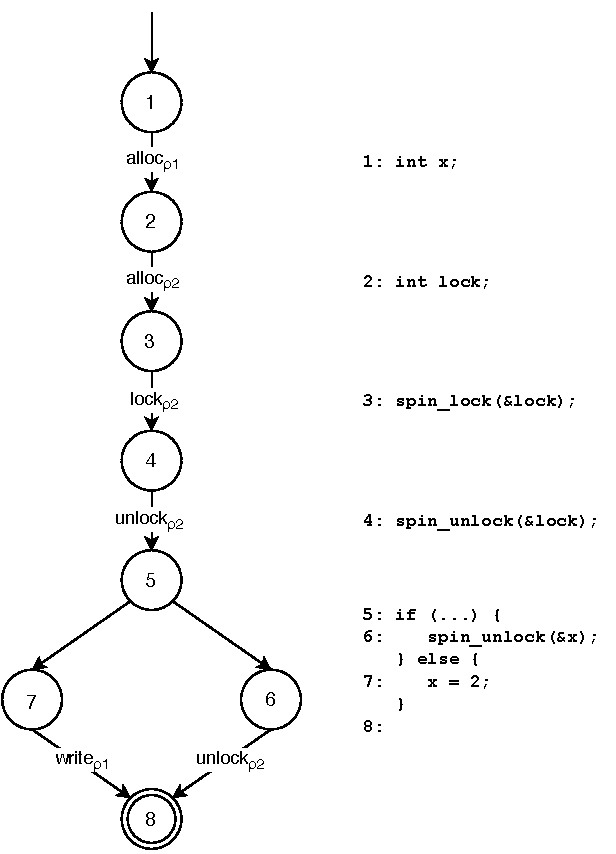
\includegraphics[width=0.5\textwidth]{algorithm/figures/cfg_example}
    \caption{An illustration of a Control Flow automaton.}
    \label{cfg_example-automaton}
\end{figure}

\begin{itemize}
    \item $s_0 = Entry$ 
    \item {
        $
            \begin{aligned}[t]
            \delta = \text{the relation} \; \{ \; & (Entry, (\texttt{alloc},\rho), (allocated, \rho)), \\ 
            & (allocated, (\texttt{alloc},\rho), (allocated, \rho)), \\ 
            & ((allocated, \rho), (\texttt{lock}, \rho), (locked, \rho)), \\
            & ((locked, \rho), (\texttt{unlock}, \rho), (unlocked, \rho)), \\
            & ((unlocked, \rho), \texttt{unlock}, (unlocked, \rho), \\ 
            & ((write, \rho), \texttt{write}, (written, \rho)), \\ 
            & ((unlocked, \rho), \texttt{Nil}, End), \\ 
            & ((written, \rho), \texttt{Nil}, End) \; \}
            \end{aligned}
        $ 
    }
    \item $F = End$
\end{itemize}

\noindent A few things are of note here; $Nil$ indicates the end of a path in the tree structure. Branches occur when an if-branch is encountered in the input source file and models the effects of the statements within if-statements.

\newpar To show the detection of a possible double-unlock bug where a double-unlock monitor automaton has reached the final state, we find the product of the control flow example shown in Figure \ref{cfg_example-automaton} and the monitor generated from the template. 

\newpar Given two automata $A_{CFG} = (\sum, S, s_0, \delta, F)$ and $A_{monitor} = (\sum, S', s'_0, \delta', F')$ both working over the same alphabet $\sum$, the product automaton of $A_{CFG}$ and $A_{monitor}$ is an automaton $P = (\sum, Q, s'_0, \delta_P, F_P)$ where $F_N = S \times F' \cup F \times S'$, $Q = S \times S'$ and $\delta_P : Q \times \sum \rightarrow Q$. Furthermore, $\forall q \in Q , q' \in Q'$ and $e \in \sum$, we require that since monitors generated from the monitor template only monitor a given input region, it is necessary to define rules for the state changes within this product, given that a monitor only accepts effects on a given region. This requirement can be formalized as follows.

\begin{center}
    \begin{prooftree}
        \hypo{s \xrightarrow{e} s'}
        \hypo{p \xrightarrow{E} p'}
        \hypo{e \in E}
        \infer3{(s, p) \rightarrow (s', p')}
    \end{prooftree}
    \hspace{2cm}
    \begin{prooftree}
        \hypo{p \xrightarrow{E} p'}
        \hypo{\forall e \in E\:.\:s \centernot{\xrightarrow{e}}}
        \infer2{(s, p) \rightarrow (s, p')}
    \end{prooftree}
\end{center}
    
\newpar $E$ is the set of effects happening in a given program step, $p \rightarrow p'$. The state $s$ will change given that the transition happens on the effect $e$, present in $E$. If this is not the case, the control flow will have changed state to $p'$, while the monitor has not and stays the same, $s$. 

\newpar In other words, the state of the automata should not change if the effect does not happen on the monitored region, but the automaton representing the control flow \textit{should}. The observant reader might notice that if regions are no longer present since they go out of scope scope in a given program, only the rightmost of the two previous inference rules is relevant. This is not the case though, since the previous control flow abstraction does not provide any information in regards to when variables go out of scope, mirroring the internal control flow representation of EBA. Furthermore, taking scopes into account would complicate the product construction significantly and the reader might appreciate not having to reason about more convoluted definitions. Lack of scope information does lead to the question of whether these \textit{"dangling"} regions incur a performance cost when implemented. I will investigate and evaluate this in later sections. \todo{Fine? Andrzej's way of expressing this was more elegant AFAIR}  

\newpar The product of the control flow example shown in Figure \ref{cfg_example-automaton} and a generated double-unlock monitor automaton can now be found in order to demonstrate that a possible bug is detected by the monitor, resulting in the following definition. This definition is illustrated in Figure \ref{cfg_unlock-product}. 

\begin{itemize}
    \item{
        $
            \begin{aligned}[t] 
                \sum = & \{\mathit{Entry}, \mathit{Nil}, (alloc, \rho), (free, \rho), (read, \rho), \\ 
                & (write, \rho), (uninit, \rho), (call, \rho), (lock, \rho), (unlock, \rho)\}
            \end{aligned} 
        $
    }
    \item{
        $
            \begin{aligned}[t]
                S = & \{(allocated, \rho), (freed, \rho), (read, \rho), (written, \rho),\\ 
                & (uninitialized, \rho), (called, \rho), \\
                & ((locked, \rho), locked_\rho), ((unlocked, \rho), unlocked_\rho), \\
                & ((unlocked, \rho), error_\rho), \\
                & End\}
            \end{aligned}
        $
    }
    \item $s_0 = Entry$ 
    \item {
        $
            \begin{aligned}[t]
            \delta = \text{the relation} \; \{ \; & (Entry, (\texttt{alloc},\rho), (allocated, \rho)), \\ 
            & (allocated, (\texttt{alloc},\rho), (allocated, \rho)), \\ 
            & ((allocated, \rho), (\texttt{lock}, \rho), (locked, \rho)), \\
            & ((locked, \rho), (\texttt{unlock}, \rho), ((unlocked, \rho), unlocked_\rho), \\
            & (((unlocked, \rho), unlocked_\rho), \texttt{unlock}, ((unlocked, \rho), error_\rho)), \\ 
            & (((write, \rho), unlocked_\rho), \texttt{write}, ((written, \rho), unlocked_\rho)), \\ 
            & (((unlocked, \rho), error_\rho), \texttt{Nil}, (End, error_\rho)), \\ 
            & (((written, \rho), unlocked_\rho), \texttt{Nil}, (End, error_\rho)) \; \}
            \end{aligned}
        $ 
    }
    \item $F = (End, error_\rho)$  
\end{itemize}

\noindent This product is illustrated in Figure \ref{cfg_unlock-product}. 

\begin{figure}[H]
    \centering
    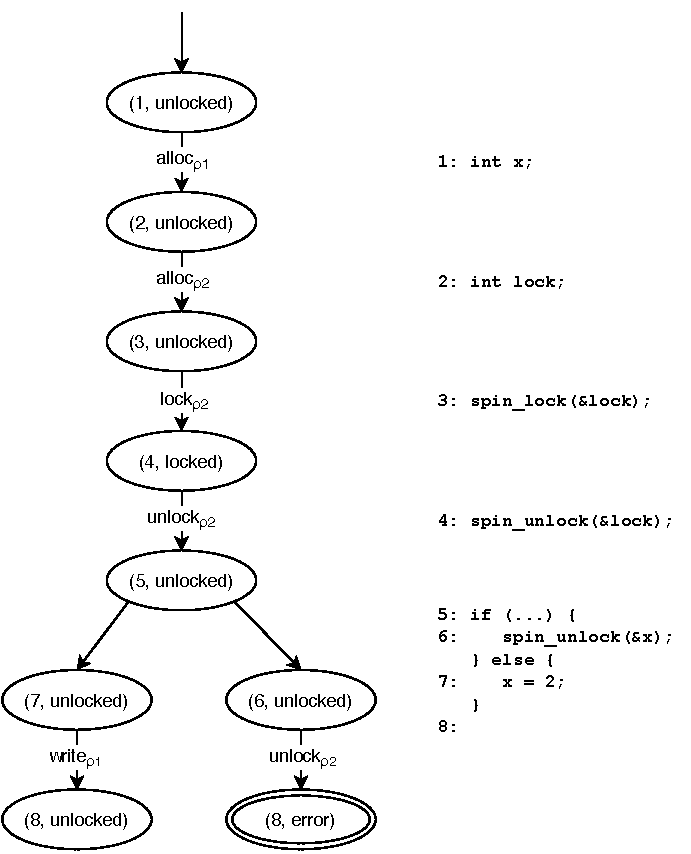
\includegraphics[width=0.5\textwidth]{algorithm/figures/cfg_unlock-product}
    \caption{An illustration of the product construction of a double-unlock monitor automata and a control flow.}
    \label{cfg_unlock-product}
\end{figure}

\newpar I have shown that it is possible to construct monitor templates which allows generating monitor automata monitoring effects happening on a region and shown that such a monitor can detect a possible bug in an example control flow. In order to implement this approach in practice, two things are needed, namely

\begin{itemize}
    \item A control flow abstraction
    \item Concrete definitions of monitor templates
\end{itemize}

\noindent It is therefore necessary to implement these monitor templates, since the EBA framework can provide the control flow abstractions over a given input file. I will present the implemetation of the monitor templates as part of this thesis in the following section. 